
\section{觀念與公式}

\subsection{多項式定義與運算}
多項式是變數與係數的代數式,形式為:
\[
P(x) = a_n x^n + a_{n-1} x^{n-1} + \cdots + a_1 x + a_0, \quad a_n \neq 0
\]
$n$為次數。\\
\textbf{運算}:
\begin{itemize}
    \item 加減:同次項合併。
    \item 乘法:分配律,如$(x + 1)(x - 2) = x^2 - x - 2$。
    \item 除法:$P(x) = Q(x)D(x) + R(x)$,$R(x)$次數低於$D(x)$。
    \item \textbf{綜合除法}:快速除以$(x - a)$,如$P(x) = x^3 - 3x^2 + 2$除以$(x - 1)$:
    \[
    [1, -3, 0, 2] \xrightarrow{1} [1, -2, -2, 0], \quad \text{商} x^2 - 2x - 2, \text{餘數} 0
    \]
\end{itemize}
\textbf{應用}:簡化、找根。\\
\textbf{大學技巧}:綜合除法比長除法高效。

\subsection{餘數定理與因式分解}
\textbf{餘數定理}:$P(x)$除以$(x - a)$,餘數為$P(a)$。若$P(a) = 0$,則$(x - a)$為因式(因式定理)。\\
\textbf{因式分解}:
\begin{itemize}
    \item 提公因式:$2x^2 + 4x = 2x(x + 2)$。
    \item 公式:$x^3 - y^3 = (x - y)(x^2 + xy + y^2)$。
    \item 試根法:用$P(a) = 0$找根,再分解。
\end{itemize}
\textbf{餘數關係延伸}:$P(x)$除以二次式$ax^2 + bx + c$,餘數為$rx + s$,可用待定係數法求解。\\
\textbf{應用}:驗證根、分解多項式。\\
\textbf{大學技巧}:用微分確認根重數,若$P'(a) = 0$,$a$為重根。

\subsection{根與係數關係}
對於$P(x) = a_n x^n + \cdots + a_0$,根$r_1, r_2, \ldots, r_n$滿足(Vieta's公式):
\[
\sum r_i = -\frac{a_{n-1}}{a_n}, \quad \sum r_i r_j = \frac{a_{n-2}}{a_n}, \quad \prod r_i = (-1)^n \frac{a_0}{a_n}
\]
如$x^3 - 6x^2 + 11x - 6$,根和$6$,乘積$6$。\\
\textbf{應用}:求未知係數、驗證根。\\
\textbf{大學技巧}:結合微分分析根的分布。

\subsection{微分與局部特徵}
\textbf{導數}:
\begin{itemize}
    \item $P'(x)$:斜率,$P'(x) = 0$為極值點。
    \item $P''(x)$:凹凸性,$P''(x) > 0$為凹向上。
    \item 重根:$P(a) = P'(a) = 0$,$P''(a) \neq 0$為二重根。
\end{itemize}
\textbf{局部特徵}:單根改變符號,重根不變。\\
\textbf{應用}:極值、單調性。\\
\textbf{大學技巧}:$P^{(k)}(a)$判斷$k$重根。

\subsection{泰勒展開與廣域特徵}
\textbf{泰勒展開}:$P(x)$在$x = a$:
\[
P(x) = P(a) + P'(a)(x - a) + \frac{P''(a)}{2!}(x - a)^2 + \cdots + \frac{P^{(n)}(a)}{n!}(x - a)^n
\]
如$x^3 - x$在$x = 0$,$P(x) = -x + x^3$。\\
\textbf{廣域特徵}:
\begin{itemize}
    \item $n$次多項式有$n$個根(含重根)。
    \item $x \to \pm \infty$,$P(x)$由$a_n x^n$決定。
\end{itemize}
\textbf{應用}:近似、趨勢分析。\\
\textbf{大學技巧}:泰勒展開快速估計局部值。

\subsection{牛頓插值法}
用點$(x_i, y_i)$插值:
\[
P(x) = f(x_0) + f[x_0, x_1](x - x_0) + f[x_0, x_1, x_2](x - x_0)(x - x_1) + \cdots
\]
差商:$f[x_0, x_1] = \frac{f(x_1) - f(x_0)}{x_1 - x_0}$。\\
\textbf{應用}:數據擬合。\\
\textbf{大學技巧}:比拉格朗日插值更高效。

\section{例題解析}

\subsection{例題1:餘數定理}
求$x^3 - 2x^2 + x - 1$除以$(x - 2)$的餘數。\\
\textbf{解}:$P(2) = 8 - 8 + 2 - 1 = 1$。綜合除法驗證:
\[
[1, -2, 1, -1] \xrightarrow{2} [1, 0, 1, 1], \quad \text{餘數} 1
\]
\textbf{大學技巧}:餘數定理直接得出。

\subsection{例題2:根與係數}
若$x^3 - kx^2 + 5x - 2 = 0$的根和為$3$,求$k$。\\
\textbf{解}:$\sum r_i = \frac{k}{1} = 3$,$k = 3$。\\
\textbf{大學技巧}:試根$P(1) = 2$,調整驗證。

\subsection{例題3:泰勒展開}
求$x^3 - 3x + 1$在$x = 1$的泰勒展開(至二階)。\\
\textbf{解}:$P(1) = -1$,$P'(x) = 3x^2 - 3$,$P'(1) = 0$,$P''(x) = 6x$,$P''(1) = 6$:
\[
P(x) = -1 + 0(x - 1) + 3(x - 1)^2
\]
\textbf{大學技巧}:全展開等於原式。

\subsection{例題4:牛頓插值}
用點$(0, 1), (1, 0), (2, 3)$插值。\\
\textbf{解}:差商:
\[
f[0, 1] = -1, \quad f[1, 2] = 3, \quad f[0, 1, 2] = 2
\]
\[
P(x) = 1 - x + 2x(x - 1) = 2x^2 - 3x + 1
\]
\textbf{大學技巧}:驗證點值吻合。

\section{圖形展示}
$x^3 - 3x + 1$:
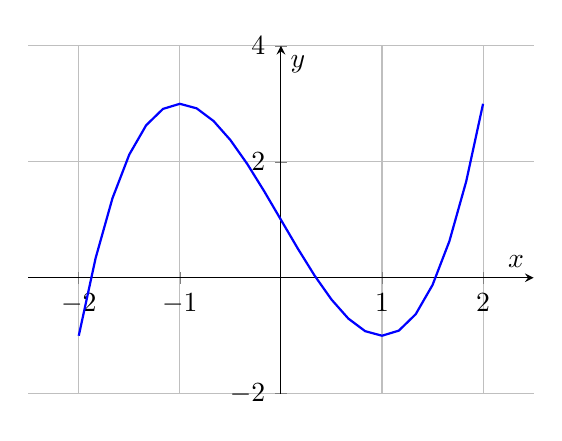
\begin{tikzpicture}
    \begin{axis}[
        axis lines=middle,
        xlabel=$x$,
        ylabel=$y$,
        xmin=-2.5, xmax=2.5,
        ymin=-2, ymax=4,
        grid=both,
        width=8cm, height=6cm
    ]
    \addplot[domain=-2:2, blue, thick] {x^3 - 3*x + 1};
    \end{axis}
\end{tikzpicture}

\section{題庫}
\begin{enumerate}[label=\arabic*.]
    % 計算題 (10)
    \item 計算$(x + 1)(x^2 - 2x + 1)$。
    \item 分解$x^3 - 8$。
    \item 求$x^3 - 3x^2 + 2x - 1$除以$(x - 1)$的餘數。
    \item 分解$x^4 - 16$。
    \item 若$P(x) = x^3 - 2x + 1$,求$P(2)$。
    \item 用綜合除法求$x^3 - 4x^2 + 5x - 2$除以$(x - 2)$的商。
    \item 分解$x^2 - 4x + 4$。
    \item 求$x^3 - x + 1$在$x = 0$的泰勒展開(至二階)。
    \item 若$P(x) = x^3 + x^2 - x - 1$,求$P(-1)$。
    \item 分解$x^3 + 27$。
    % 應用題 (10)
    \item 求$x^3 - 3x^2 + 3x - 1$的實根與重數。
    \item 若$P(x) = x^3 - 5x^2 + kx - 2$根和為$5$,求$k$。
    \item 求$x^3 - 2x + 1$在$[0, 1]$的最小值。
    \item 用點$(0, 0), (1, 1), (2, 0)$插值多項式。
    \item 求$x^4 - 4x^2 + 3$的極值點。
    \item 若$P(x) = x^3 - 6x^2 + 11x - 6$,求根的乘積。
    \item 求$x^3 - x^2 + x - 1$在$[-1, 1]$的最大值。
    \item 若$P(x) = x^3 + 2x^2 - 5x - 6$,求單調區間。
    \item 求$x^3 - 3x + 2$的廣域趨勢。
    \item 若$P(x) = x^4 - 2x^2 + 1$,求$P''(x)$的根。
    % 觀念題 (10)
    \item 證明餘數定理:$P(x) = (x - a)Q(x) + P(a)$。
    \item 若$P(x)$有二重根,$P'(a)$如何?
    \item 說明根與係數關係的應用。
    \item 若$P(x)$為三次多項式,實根數可能為何?
    \item 證明泰勒展開對於多項式的有限項。
    \item 說明綜合除法如何找根。
    \item 若$P(x)$趨向負無窮,$a_n$如何?
    \item 證明$x^3 - x + 1$至多1實根。
    \item 說明牛頓插值如何保證唯一。
    \item 若$P(x)$除以$(x^2 + 1)$,餘數形式為何?
    % 進階題 (10)
    \item 求$x^3 - 4x^2 + 5x - 2$的所有實根。
    \item 若$P(x) = x^4 - 5x^2 + 4$,求極值。
    \item 求$x^3 - 6x^2 + 9x - 4$的局部特徵。
    \item 用綜合除法求$x^3 - 2x^2 + x - 1$除以$(x - 1)$的商。
    \item 求$x^3 + 2x^2 - x - 2$在$x = 1$的泰勒展開(至一階)。
    \item 若$P(x) = x^3 - 3x^2 + 2x - 1$,求$P'(x)$的根。
    \item 求$x^4 - 2x^3 + x^2 - 2x + 1$的實根數。
    \item 若$P(x) = x^3 - x^2 - x + 1$,求廣域特徵。
    \item 用點$(0, 1), (1, 2), (2, 5)$插值多項式。
    \item 求$x^3 - 5x^2 + 8x - 4$的根與重數。
    % 挑戰題 (20)
    \item 若$P(x) = x^4 - 4x + 3$,求所有實根與極值。
    \item 求$x^3 - 3x^2 + 3x - 1$在$x = 1$的泰勒展開(至三階)。
    \item 若$P(x) = x^5 - 5x + 4$,求實根數。
    \item 求$x^3 - 4x^2 + 5x - 2$的餘數關係(除以$x - 3$)。
    \item 若$P(x) = x^4 - 2x^2 - 3$,求極值與根。
    \item 求$x^3 + 2x^2 - 5x - 6$的所有實根。
    \item 用綜合除法分解$x^4 - 3x^3 + 2x^2 - x + 1$除以$(x - 1)$。
    \item 若$P(x) = x^3 - x^2 - x + 1$,求$x \in [-1, 1]$的最小值。
    \item 求$x^3 - 6x^2 + 11x - 6$的根與係數關係。
    \item 用點$(0, 0), (1, 1), (2, 4)$插值多項式。
    \item 若$P(x) = x^4 - 2x^3 + x^2 - 2x + 1$,求極值。
    \item 求$x^3 - 3x^2 + 2x - 1$在$[0, 1]$的最大值。
    \item 若$P(x) = x^3 + x^2 - 2x - 2$,求單調區間。
    \item 求$x^4 - 4x^2 + 3$在$[0, 2]$的最大值。
    \item 若$P(x) = x^3 - 2x^2 - 5x + 6$,求$P''(x)$的根。
    \item 求$x^3 - 5x^2 + 8x - 4$在$x = 1$的泰勒展開(至二階)。
    \item 若$P(x) = x^4 - x^2 + 1$,求廣域特徵。
    \item 求$x^3 + 3x^2 - 4x - 12$的所有實根。
    \item 用綜合除法求$x^3 - 4x^2 + 3x + 1$除以$(x - 2)$的商。
    \item 若$P(x) = x^5 - x^3 + x - 1$,求$x \in [0, 1]$的最小值。
\end{enumerate}
